\section{Maschine Learning}

Der Fokus dieser Arbeit ist die Ermittlung von Design von Quellcode durch die Anwendung von Maschine Learning.
Dieser Teil der Arbeit ist für die Erläuterung von verwendeten Metriken, angewandten Techniken und ausgewählter Klassifizierer gewidmet.

% TODO: \subsection{Terminologie} falls notwendig
\subsection{Metriken für Evaluierung von Modellen}\label{metrics}

Um die Leistung eines Klassifizierers zu ermitteln, bedarf es einer Menge an Metriken, womit beurteilt werden, ob der Klassifizierer wie erwartet performt.
In Kontext dieser Aussage wird in der Domäne des Maschine Learnings bekannte Metriken aus dem Bereich der Statistik angewendet.
In diesem Abschnitt wird eine Auswahl von solchen Metriken erläutert, die in der Literaturrecherche als auch in den Sektionen der Methodik und Implementierung erwähnt werden.
Für die Ermittelung der Metriken werden folgende Größen definiert:

\begin{description}
    \item TP (True Positive): Anzahl echt positiver Klassifizierungen
    \item TN (True Negative): Anzahl echt negativer Klassifizierungen
    \item FP (False Postive): Anzahl falsch positiv Klassifizierungen
    \item FN (False Negative): Anzahl falsch negativ Klassifizierungen
\end{description}

Anhand dieser Größen werden folgende Metriken definiert:

\begin{description}
    \item \textit{Accuracy (Genauigkeit)}: Dieser Wert gibt an, wie das Verhältnis zwischen den klassifizierten Beobachtungen zur Gesamtzahl der Beobachtungen ist.
    \\
    \\
    $Accuracy = \frac{\text{Anzahl der korrekten Vorhersagen}}{\text{Gesamtzahl der Vorhersagen}} = \frac{TP+TN}{TP+TN+FP+FN}$

    \item \textit{Precision (Präzision)}: Dieser Wert gibt das Verhältnis an, wie die korrekt positiv klassifizierten Beobachtungen zur Gesamtzahl der als positiv klassifizierten Beobachtungen stehen.
    \\
    \\
    $Precision = \frac{TP}{TP+FP}$

    \item \textit{Recall (Sensitivität)}: : Dies ist das Verhältnis der positiv klassifizierten Beobachtungen zur Gesamtzahl der tatsächlichen positiven Beobachtungen.
    \\
    \\
    $Recall = \frac{TP}{TP+FN}$
    
    \item \textit{ F1-Score}: Der F1-Score ist das harmonische Mittel von Präzision und Recall und gibt ein besseres Maß für die unbalancierten Klassen als die Genauigkeit allein.
    \\
    \\
    $\textit{\text{F1-Score}} = 2 * \frac{Precision * Recall}{Precision + Recall} = \frac{2*TP}{2*TP + FP + FN}$
\end{description}

\pagebreak

\subsection{Validierung und Optimierung von Modellen}

Neben dem Zusammentragen von relevanten Datenpunkte für die Erhebung eines geeigneten Datensatzes ist das Validierung und Optimierung des Maschine Learning Modells eines der relevanten Schritte im gesamten Prozess, 
um damit das Modell dessen Aufgabe möglichst zufriedenstellend erfüllen kann. 
In diesem Teil der Arbeit werden Techniken bzw. Methoden erläutert, die in der Validierungs- oder Optimierungsphase angewendet werden können.


\subsubsection{Kreuzvalidierung von Modellen}
Nach dem Trainieren des Modells für einen Datensatz ist von Interesse, wie das Modell neue unbekannte Datenpunkte umgeht und diese Leistung anhand einer Metrik zu messen.
Dies stellt den Kernpunkt der Validierungsphase dar. Ein naiver Ansatz, die gleiche Menge an Datenpunkten zu verwenden, worauf das Modell in der Trainingsphase trainiert wurde.
Dabei ist jeder Datenpunkt des Datensatzes dem Modell bereits bekannt, wodurch es nicht auf wirklich unbekannte Datenpunkte validiert.
Eine Möglichkeit dem entgegenzukommen ist das Aufteilen des Datensatzes in Trainings- und Validationsdatensatz, wobei meist der Trainingsdatensatz die größere Menge an Datenpunkten zugesprochen wird.
Jedoch besteht hier der Nachteil, das in der Trainingsphase die Datenpunkte in dem Validationsdatensatz wegfallen.
Um diesen Nachteil zu negieren, kann die Technik der Cross Validation oder Kreuzvalidierung angewendet werden.

Hierbei wird zunächst eine natürliche Zahl \textit{n} bestimmt, die angibt, in wie viele gleich große Teile der Datensatz aufgeteilt wird.
Die Trainings- und Validierungsphase wird hierbei zu einem Schritt zusammengefasst und das Modell wird iterativ \textit{n}-Mal trainiert und anhand der vorgegebenen Metrik evaluiert.

\begin{figure}[h]
    \centering
    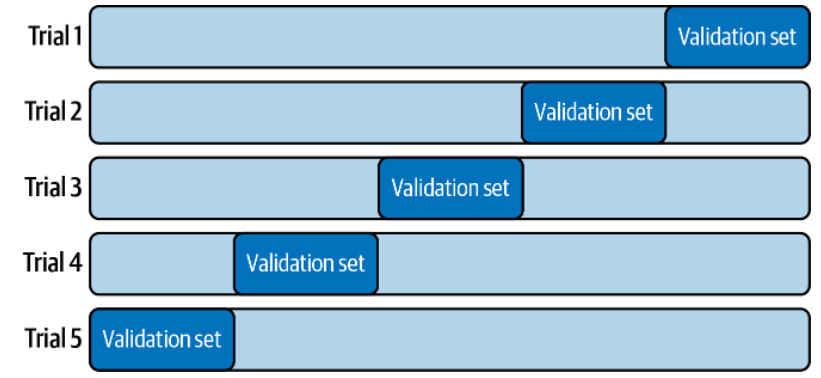
\includegraphics[scale=0.5]{figures/cross_validation}
    \caption{Kreuzvalidierung mit \textit{n} = 5}
    \label{fig:cross_validation}
\end{figure}
Wie aus Abbildung \ref{fig:cross_validation} zu entnehmen ist, wird in der \textit{i}-ten Iteration das $k-i$-te Sektion des Datensatzes für die Validierung und restlichen
für das Training des Modells verwendet. Das Resultat dieser Operation ist abhängig von Implementierung der Kreuzvalidierung die Iteration des Modells mit der besten Evaluation und eine Liste von Werten, die Leistung des Modells in der jeweiligen Iteration angibt.

\pagebreak

\subsubsection*{Optimieren von Modellen durch Hyperparameter-Tuning}\label{hyper_params}
Maschine Learning Modelle können mithilfe von Parametern konfiguriert werden. Dabei wird zwischen zwei Arten von Parametern entschieden: Modellparameter und Hyperparameter.
Modellparameter werden während der Trainingsphase automatisiert direkt durch den Trainingsdatensatz bestimmt und sind nicht von Außen zu manipulieren. Dahingegen bestimmen Hyperparameter unter anderem wie sich das Modell während der Trainingsphase zu verhalten und beeinflussen
dessen Architektur. Jedes Modell definiert hierbei selbst, welche Hyperparameter verfügbar sind. Hyperparameter werden während der Instantiierung des Modells definiert. Die Ermittelung der bestmöglichen Kombinationen an Hyperparametern-Werten ist hilfreich, falls Leistung des Modells nicht den Erwartungen entspricht und das verwendete Datensatz nicht weiter argumentiert werden kann.
Um die Leistung des Modells zu evaluieren, wird wie in der Kreuzvalidierung eine Metrik bestimmt, die Leistung der jetzigen Iterationen zu beurteilen. Das Ziel der Hyperparameter-Optimierung besteht hier darin, eine Kombination an Hyperparametern-Werten zu bestimmen, wodurch die Metrik maximiert bzw. minimiert. 
Dies kann entweder manuell durchgeführt oder es werden Methoden eingesetzt, die dies automatisiert erledigen können. Im Folgendem wird eine Auswahl an automatisierten Strategien aufgelistet und erläutert:

\begin{description}
    \item Random Search/Grid Search: In diesen Methoden werden zunächst Wertebereiche für die jeweiligen Hyperparameter bestimmt. In der Regel wird hierbei eine Menge an diskreten Wertem bestimmt, die der jeweilige Hyperparameter annehmen kann. Jede Permutation der Hyperparameter-Konfiguration wird als eine Zelle in einem Gitter erfasst. 
    Jede besuchte Zelle dient dabei als Konfiguration für eine neue Instanz des Modells, welches im weiteren Verlauf durch Einsatz von Kreuzvalidierung trainiert und evaluiert wird. Das Ergebnis der Evaluation wird vermerkt.
    Bei Random Search wird zufällig bestimmt, welche Zellen besucht werden, während bei Grid Search alle Zellen besucht werden. Das Ergebnis ist die Konfiguration des Modells mit der besten Evaluierung.
    
    \item Bayessche Optimierung: Bei Grid bwz. Random Search wird jede Permutation der Hyperparameter-Werte eine Instanz des Modells trainiert und evaluiert. Unter Umständen kann der Trainingsprozess je nach Modell und Datensatz rechenintensiv, wodurch es lange dauern, bis diese Methoden ein Resultat liefern.
    In solch einem Fall kann das Verfahren der Bayesschen Optimierung angewendet, um die Dauer der Evaluierung zu verkürzen. Im Kern wird das Maschine-Learning Modell als Black Box Funktion interpretiert, welches als Eingabe eine Permutation an Hyperparameter-Werten akzeptiert und der Wert der Zielmetrik für die jeweilige Permutation dient als Rückgabewert der Black Box Funktion.
    Dadurch, dass die Optimierung der Black Box Funktion durch Ableitungsverfahren nicht möglich, wird dieses eine Ersatzfunktion substituiert, welches die Black Box Funktion approximiert.
    Bei der Ersatzfunktion handelt es such um ein probabilistisches Modell, welches genutzt wird, um eine Wahrscheinlichkeitsverteilung über die möglichen Werte der Zielmetrik für verschiedene Kombinationen an Hyperparameter-Werten zu erstellen.
    Die Bayessche Optimierung beginnt typischerweise mit einer zufälligen Auswahl von Hyperparametern, um einige Datenpunkte zu generieren. Diese werden verwendet, um das probabilistische Modell zu initialisieren. Anschließend wird iterativ die Akquisitionsfunktion angewendet, um neue und vielversprechende Hyperparameter-Kombinationen zu identifizieren und zu testen. 
    Diese Funktion bestimmt, welche Permutation am Hyperparameter-Werten auf Basis des jetzigen Standes des probabilistischen Modells als Nächstes bewertet werden soll. 
    Sie balanciert die Exploration unbekannter Bereiche des Hyperparameterraums mit der Exploitation von Bereichen, die voraussichtlich zu besseren Ergebnissen führen.
    Nach jedem Schritt wird das Modell mit den neuen Ergebnissen aktualisiert, was zu einer kontinuierlichen Verbesserung der Schätzungen und Entscheidungen führt. Am Ende der Methode ist die Kombination an Hyperparameter-Werten bekannt, welches für die Zielmetrik das globale Minimum bzw. Maximum als Rückgabewert zurückgibt.

    \item Tree-structured Parzen Estimators (TPE): Bei TPEs handelt es sich um einen speziellen Anwendungsfall der Bayesschen Optimierung. Anstatt eine Wahrscheinlichkeitsverteilung für die Kombination an Hyperparameter-Werten zu verwenden, wird diese in zwei aufgeteilt:
    eine für Kombinationen, die zu besseren Werten für die Zielmetrik führen ("gute Verteilung") und eine für solche, die zu schlechteren Ergebnissen führen ("schlechte Verteilung"). Wie bei der normalen Bayesschen Optimierung wird eine Aquisefunktion eingesetzt, um zu bestimmen, welche Kombination an Hyperparameter-Werten als Nächstes evaluiert werden soll.
    Hierbei basiert die Akquisitionsfunktion bei TPE auf das Verhältnis der Dichten dieser beiden Verteilungen. Durch den Einsatz von Parzen Estimatoren werden für beide Wahrscheinlichkeitsverteilungen Dichtefunktionen approximiert, wodurch die Dichten in Akquisitionsfunktion bestimmt werden können.
    Sie wählt die nächste zu evaluierende Hyperparameter-Kombination, indem sie Bereiche bevorzugt, in denen das Verhältnis der Dichte der "guten" Verteilung zur Dichte der "schlechten" Verteilung hoch ist.
    Wie in der normalen Bayesschen Optimierung wird das probabilistische Modell iterativ mit neuen Werten aktualisiert, um ein globales Minimum bzw. Maximum der Black Box Funktion zu ermitteln.

\end{description}

\pagebreak
%%TODO: Add references from literature

\subsection{Betrachtete Klassifizierer} \label{classifiers}
Für die Bestimmung eines Design Patterns wird eine Menge an Rollen bestimmt, die die Submuster innerhalb des jeweiligen Entwurfsmusters erfüllen.
Die Bestimmung der Rollen für einzelne Submuster fällt in dem Bereich des Maschine-Learnings in den Bereich der Klassifikation. Im Sinne dieser werden in diesem Abschnitt der Arbeit eine Auswahl von Klassifizierern betrachtet und erläutert,
die im Kontext dieser Arbeit in Anbetracht gezogen werden.

\subsubsection*{Support Vector Maschines}

Support Vector Mashines oder SVMs sind überwachte Maschine-Learning Modelle, die sowohl für Regressions- als auch für Klassifikationsaufgaben einsetzbar ist. Die Datenpunkte werden in einen \textit{n}-dimensionalen Raum abgebildet, wobei \textit{n} die Anzahl der Features der Datenpunkte beschreibt.
Bei der Klassifizierung trennen SVMs den Raum der Datenpunkte in verschiedene Zonen. Jede Zone entspricht einem Label, zu welchen die Datenpunkte in der jeweiligen Zone zugeordnet werden. Die Grenzen der einzelnen Zonen werden durch Hyperplanes beschrieben. Das Ziel ist, diese Hyperplanes so zu bestimmen,
sodass die Datenpunkte möglichst distinkt einer Zone zugeordnet werden.

\begin{figure}[h]
    \centering
    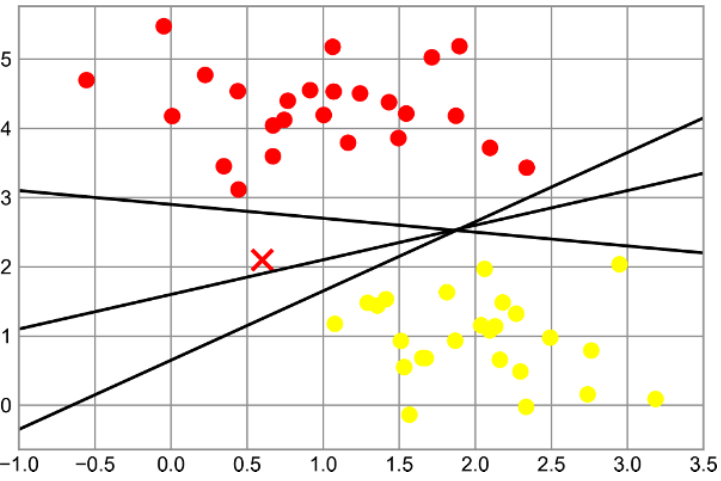
\includegraphics[scale=0.5]{figures/support_vector_new_point.png}
    \caption{Grafische Darstellung einer SVM im zwei-dimensionalen Raum}
    \label{fig:svm_graphic}
\end{figure}

Abbildung \ref{fig:svm_graphic} grafisch, wie eine SVM funktioniert. Punkte sind die Datenpunkte des Datensatzes und die Farben der Punkte die Klasse, in der die Punkte eingeordnet sind.
Die Linien beschreiben die mögliche Hyperplanes, womit Grenzen zwischen den Klassen determiniert wird. Das Kreuz zeigt einen neuen Datenpunkt, der zu klassifizieren ist. Mit diesem neuen Datenpunkt stellt sich die Frage, welche der drei möglichen Hyperplanes zu wählen ist, um die Datenpunkte möglichst distinkt einer Klasse zuzuordnen.

\pagebreak

\begin{figure}[h]
    \centering
    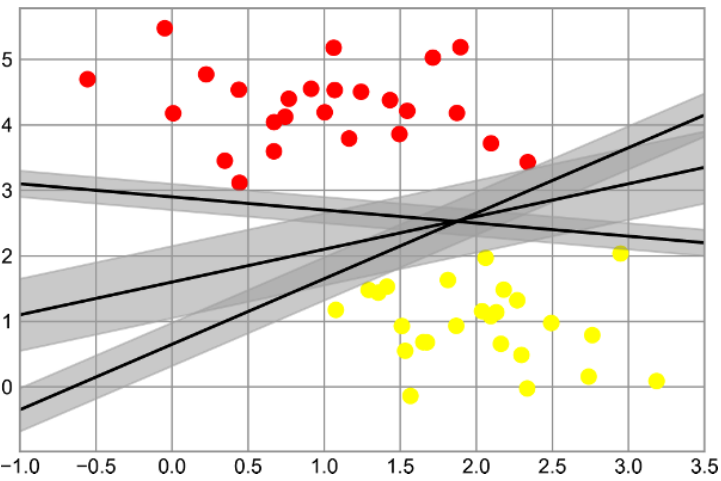
\includegraphics[scale=0.5]{figures/support_vector_maschine_margins.png}
    \caption{Hyperplanes mit Margen}
    \label{fig:svm_margins}
\end{figure}

Wie in Abbildung \ref{fig:svm_margins} zu sehen ist, wird für jede Hyperplane die Marge zwischen der Hyperplane und der Datenpunkte und den nächsten Datenpunkten bestimmt.
Die Hyperplane mit der größten Marge, die mit der größten Distanz zwischen sich und den nächsten Datenpunkten, wird als finale Hyperplane für die Grenzbildung zwischen den Klassen gewählt. Im Falle von Abbildung \ref{fig:svm_margins}
ist dies mittlere von den drei Kandidaten. Mit jedem neuen Datenpunkt wird währed Trainings wird die ideale Hyperplane neu bestimmt.
Jedoch stellt sich die Frage, wie mit Datensätzen umzugehen, die nicht durch lineare Hyperplanes in Klassen aufgeteilt werden.

\pagebreak

\begin{figure}[h]
    \centering
    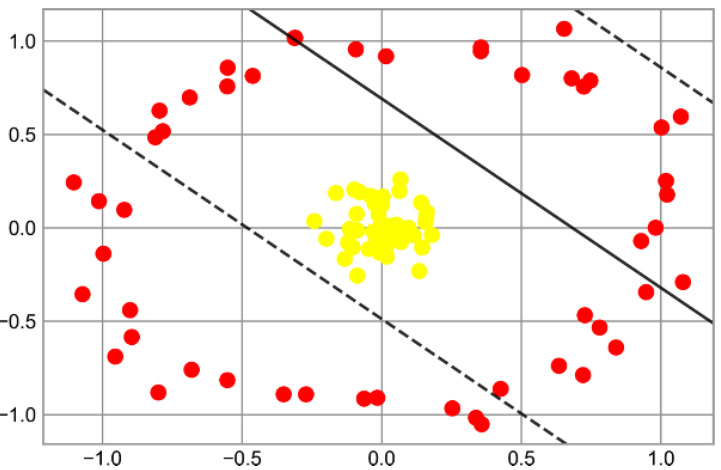
\includegraphics[scale=0.5]{figures/svm_non_linear.png}
    \caption{Nicht mögliche Einteilung durch lineare Hyperplanes}
    \label{fig:svm_non_linear}
\end{figure}


Abbildung \ref{fig:svm_non_linear} zeigt einen Datensatz, dessen Datenpunkte nicht distinkt durch lineare Hyperplanes zugeordnet werden können. Um trotzdem lineare Hyerplanes zu bilden,
wird der bei SVMs Kernel verwendet. Bei dem Kernel Trick handelt es sich um eine Funktion, die den Datensatz in einen Raum mit einer höheren Dimension projektiert.
Durch die Projektion in einem Raum mit einer höheren Dimension ist es möglich, lineare Hyperplanes zu bestimmen.
Diese Funktion werden als Kernel bezeichnet und werden bei der Instantiierung des Modells als Hyperparameter mitgegeben.

\begin{figure}[h]
    \centering
    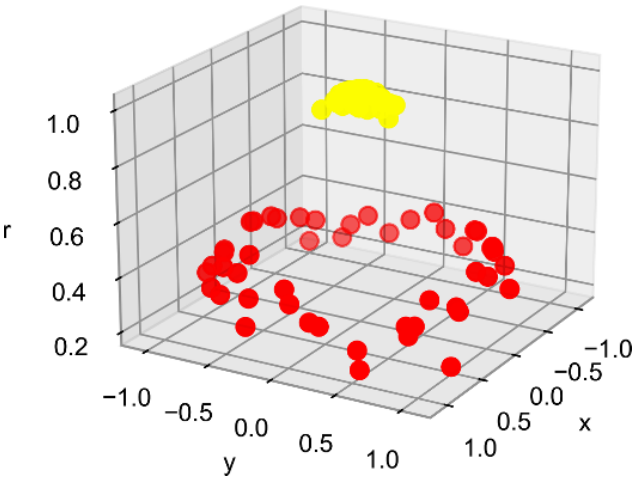
\includegraphics[scale=0.5]{figures/svm_kernel_transformation.png}
    \caption{Transformierter Datensatz aus Abbildung \ref{fig:svm_non_linear} durch RBF}
    \label{fig:svm_transformed}
\end{figure}

Abbildung \ref{fig:svm_transformed} zeigt, wie durch Anwendung des Radial-Basis-Function Kernel, das den ursprünglich zwei-dimensionalen Raum auf ein drei-dimensionales projektiert wird.
Durch die Transformation kann nun eine Hyperplane als Ebene bestimmt werden, wodurch die Klassifikation ermöglicht wird.

\pagebreak

\subsubsection*{k-Nearest Neighbor Classifier}

k-Nearest Neighbors Classifier oder KNN kann wie die SVM für Regressions- als auch für Klassifikationsprobleme eingesetzt werden. Dabei wird bei KNN unter der Annahme agiert, dass ähnliche Datenpunkte in der Nähe zueinander sind.
Der Hyperparameter k definiert die Anzahl der nächsten Nachbarn, die verwendet werden, um den neu eingefügten Datenpunkten eine Klasse zuzuordnen. Um die k nächsten benachbarten Datenpunkte zu identifizieren, ist ein Maß erforderlich, welches die Distanz zwischen diesen beschreibt. Dieses wird als Hyperparameter bei des Instantiierung des Modells diesem übergeben.
Folgende Größen können als Metrik für die Distanz verwendet werden:

\begin{description}
    \item Euklidische Distanz ist die Länge des Liniensegmentes zwischen den beiden Punkten im euklidischen Raum.
    \\
    \begin{math}
        d_{euclidean} (P, Q)= \sqrt{(p_1 - q_1)^2 + (p_2 + q_2)^2 + \ldots + (p_n - q_n)^2}
        \\
        \\
        \text{mit}
        \\
        \\
         P = (p_1, p_2, \ldots, p_n)
         \\
         Q = (q_1, q_2, \ldots, q_n)
    \end{math}
    
    \item Manhattan Distanz ist die Summe der absoluten Differenz zwischen den Komponenten der Punkte.
    \\
    \begin{math}
        d_{manhatten} (P, Q) = |p_1 - q_1| + |p_2 - q_2| + \ldots + |p_n - q_n|
        \\
        \\
        \text{mit}
        \\
        \\
         P = (p_1, p_2, \ldots, p_n)
         \\
         Q = (q_1, q_2, \ldots, q_n) 
    \end{math}
    \item Minkowski Distanz ist eine allgemeinere Metrik, um die Distanz zwischen zwei Punkten im n-dimensionalen Raum zu ermitteln.
    \\
    \begin{math}
        d_{minkowski}(P, Q) = (|p_1 - q_1|^p + \ldots + |p_n - q_n|^p)^\frac{1}{p}
        \\
        \\
        \text{mit}
        \\
        \\
         P = (p_1, p_2, \ldots, p_n)
         \\
         Q = (q_1, q_2, \ldots, q_n)
         \\
         p = \text{Typ der zu kalkulierenden Distanz ($p = 1$ --> Manhatten Distanz, $p = 2$ --> Euklidische Distanz)} 
    \end{math}
\end{description}
Die Klassifizierung des neuen Datenpunktes erfolgt im Kontext der k nächsten benachbarten Datenpunkte. Die Klasse, welche am häufigsten in den k benachbarten Punkten vorkommt, wird dem neuen Datenpunkt zugewiesen.

\pagebreak

\subsubsection*{Random Forest Classifier}
Der Random Forest Classifier ist ein mächtiges, ensemble-basiertes Lernverfahren im Bereich des maschinellen Lernens, das für Regressions- und Klassifizierungsaufgaben eingesetzt wird. Es kombiniert die Vorhersagen mehrerer Entscheidungsbäume, um zu einer endgültigen Entscheidung zu kommen, wobei es sich durch hohe Genauigkeit und die Fähigkeit auszeichnet, Overfitting zu vermeiden.
Overfitting beschreibt dabei das Phänomen, bei dem ein Modell zu stark an die spezifischen Details und das Rauschen des Trainingsdatensatzes angepasst ist, sodass das Erkennen zugrundeliegenden Mustern nicht erfasst wird.
Das grundliegende Element in einem Random Forest Classifier stellen die Decision Trees oder Entscheidungsbäume, die in Summe den "Wald" des Random Forest Classifiers bilden. Diese werden während des Trainings erzeugt.
Ein Entscheidungsbaum ist dabei ein Modell, das Entscheidungen und deren mögliche Konsequenzen, einschließlich Zufallsereignissen, Kosten und Nutzen, in Form eines Baumdiagramms darstellt. Ein Entscheidungsbaum besteht aus Knoten, die Testfragen oder -kriterien repräsentieren, und Blättern, die die Endentscheidungen oder Ausgänge darstellen. Die Auswahl eines Pfades von der Wurzel bis zu einem Blatt repräsentiert eine Reihe von Entscheidungen, die zu einem bestimmten Ergebnis führen.
Die Ergebnisse der einzelnen Entscheidungsbäume werden zu einem Gesamtergebnis aggregiert. Folgende Hauptkonzepte erhöhen dabei dessen Effektivität:

\begin{itemize}
    \item Bagging (Bootstrap Aggregating): Jedem Entscheidungsbaum im Random Forest Classifier wird aus einer zufälligen Auswahl von Trainingsdaten mit Zurücklegen gebildet. Dieser Prozess führt zu unterschiedlichen Bäumen, die unterschiedliche Aspekte der Daten erfassen.
    \item  Bei der Aufteilung eines Knotens während der Baumkonstruktion wird eine zufällige Auswahl von Merkmalen betrachtet. Diese Technik trägt zur Diversifizierung der Entscheidungsbäume bei und verringert die Korrelation zwischen den Bäumen, wodurch das Modell robuster gegenüber Overfitting wird.
\end{itemize}

%%TODO